\chapter{Bevindingen van het proof of concept}\label{chap:q2}
Dit hoofdstuk presenteert de bevindingen die zijn waargenomen tijdens het uitvoeren van het experiment waaruit de vraag \researchQuestionThree (\textbf{SRQ3} uit paragraaf \ref{chap:researchQuestions}) word beantwoord.

\section{The good}
\begin{itemize}
  \item Reliability en speed is top.
  \item Traceability van transacties is top.
\end{itemize}

\section{The bad}
\begin{itemize}
  \item Technologie is nog niet mature genoeg.
  \item Smart contracts nog te beperkt.
\end{itemize}

\newpage

\section{Het resultaat}
\begin{figure}[h!]
    \begin{center}
        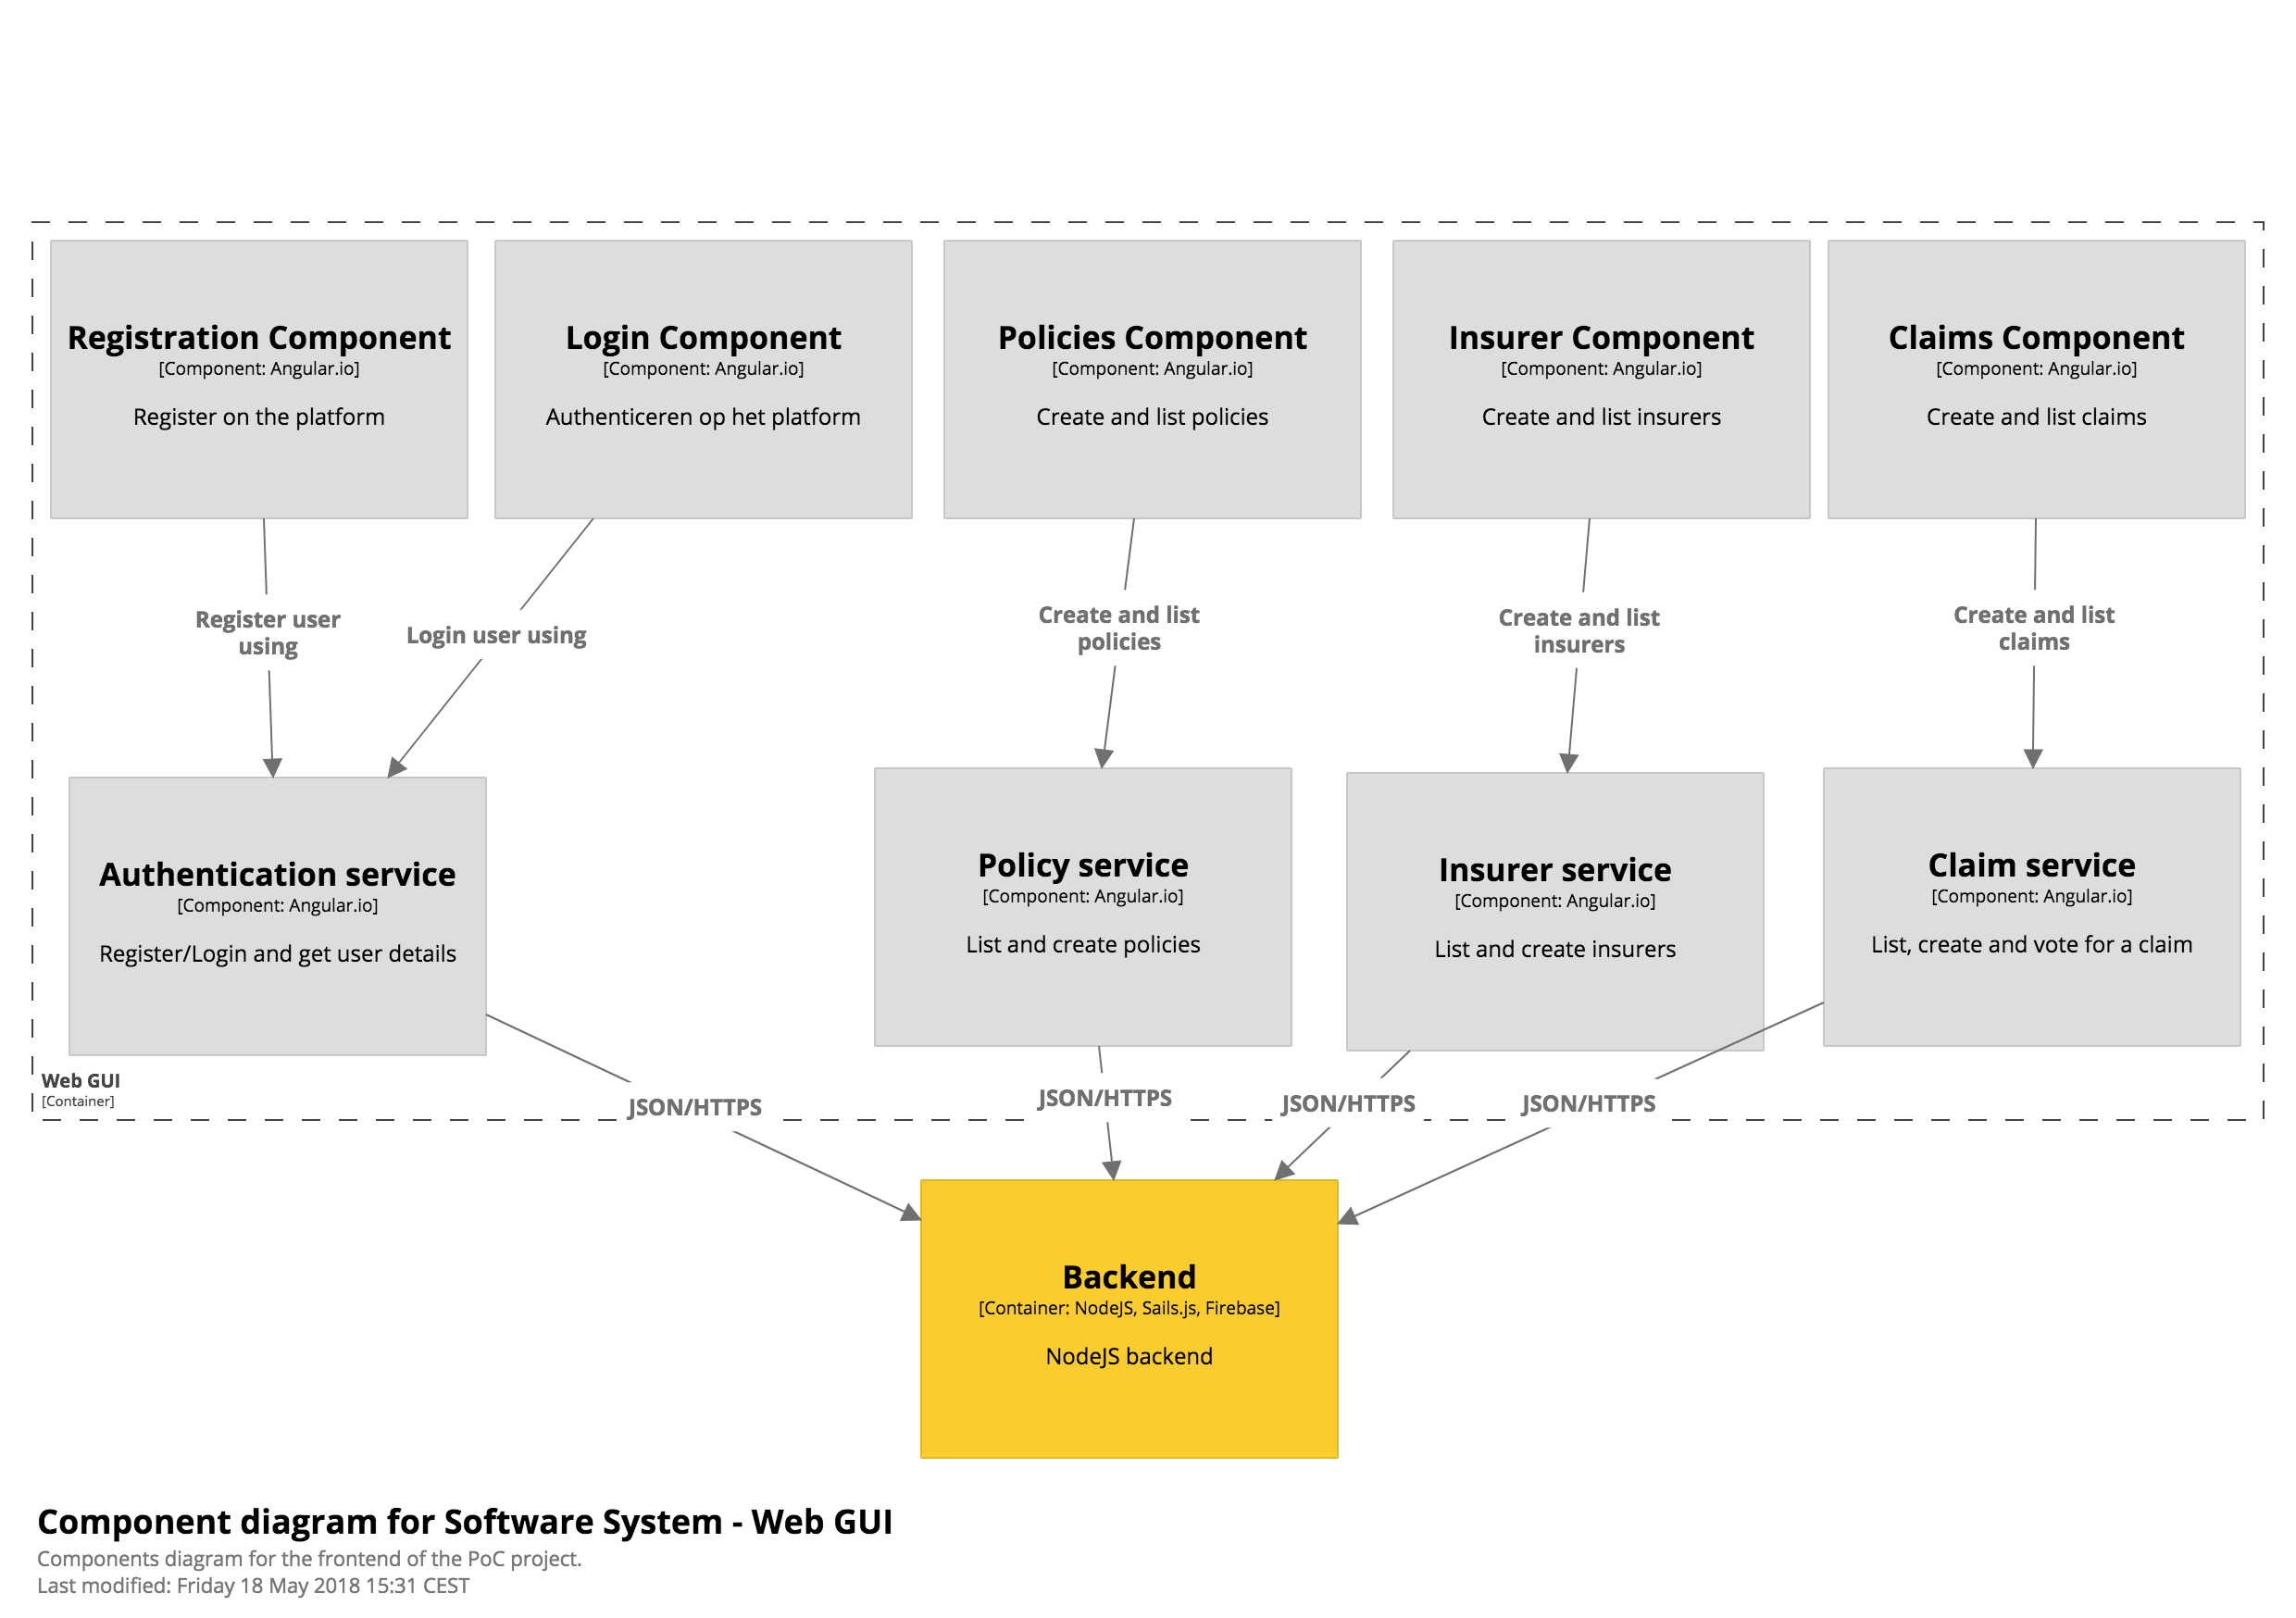
\includegraphics[width=\paperwidth-200]{images/components}
        \caption{C4 - Components.}
        \label{fig:c4Compomnents}
    \end{center}
\end{figure}